%--------------------
% Packages
% -------------------
\documentclass[11pt,a4paper,titlepage]{article}
\usepackage[utf8x]{inputenc}
\usepackage[T1]{fontenc}
%\usepackage{gentium}
\usepackage{mathptmx} % Use Times Font


\usepackage[pdftex]{graphicx} % Required for including pictures
\usepackage[english]{babel} % Swedish translations
\usepackage[pdftex,linkcolor=black,pdfborder={0 0 0}]{hyperref} % Format links for pdf
\usepackage{calc} % To reset the counter in the document after title page
\usepackage{enumitem} % Includes lists

\frenchspacing % No double spacing between sentences
\linespread{1.2} % Set linespace
\usepackage[a4paper, lmargin=0.1666\paperwidth, rmargin=0.1666\paperwidth, tmargin=0.1111\paperheight, bmargin=0.1111\paperheight]{geometry} %margins
%\usepackage{parskip}

\usepackage[all]{nowidow} % Tries to remove widows
\usepackage[protrusion=true,expansion=true]{microtype} % Improves typography, load after fontpackage is selected

%-----------------------
% Set pdf information and add title, fill in the fields
%-----------------------
\hypersetup{ 	
pdfsubject = {},
pdftitle = {},
pdfauthor = {}
}

%-----------------------
% Begin document
%-----------------------

\begin{document} %All text i dokumentet hamnar mellan dessa taggar, allt ovanför är formatering av dokumentet
\bibliographystyle{ieeetr}

\begin{titlepage}
  \centering
  \vspace*{2cm}
  {\Huge \textbf{\underline{CS-E4840}}}\\[0.5cm]
  {\Huge \textbf{\underline{\parbox{0.8\linewidth}{\centering Information Visualization D}}}}\\
  [2cm]
  {\Large Aleksi Kääriäinen (728971)}\\[0.5cm]
  {\Large \today}
\end{titlepage}

\section{Getting Started}

\subsection{SDG Selection}
\begin{enumerate}
    \item The website available at \cite{sdgs} lists \textbf{The Sustainable Development Goals} introduced by the United Nations as part of the 2030 Agenda for Sustainable Development. In total, it contains 17 goals. I selected goal number 1, i.e. the \textbf{No Poverty} goal, for the subject of visualization in this assignment.
    \item I selected the goal because it is concrete and measurable, unlike some of the other goals listed. For example, the United Nations \cite{endpov} defines the extreme poverty line to be a daily income of less than US\$2.15. This is a concrete distinction, and statistics that measure national income are commonplace, hopefully making visualization tasks simpler than with more abstract goals.
\end{enumerate}

\subsection{Visualization Analysis}
\begin{enumerate}
    \item I chose an infographic compiled by the United Nations as a visualization relating to my SDG. The visualization in figure \ref{fig:viz} is available at \cite{vizpov}.
    
    \begin{figure}[h]
        \centering
        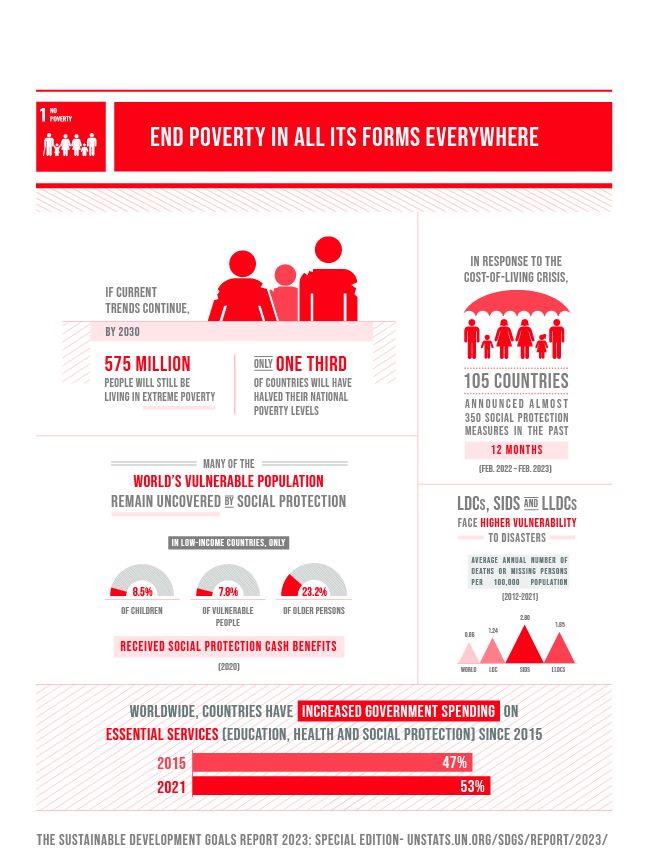
\includegraphics[width=0.4\linewidth]{reports/assignment-1/imgs/task2.jpg}
        \caption{Infographic on world poverty}
        \label{fig:viz}
    \end{figure}

    Figure \ref{fig:viz} shows the current trend for the development of the number of people living in poverty. It also shows how the poor are affected by poverty and how they are more vulnerable to disasters. On a lighter note, the infographic also shows that countries are taking concrete measures in order to reduce the number of people living in poverty.
    
    \item \begin{enumerate}
        \item Analyzing the visualization according to Tufte's principles:
        \begin{itemize}
            \item \textbf{Data-ink}
            
            The visualization presents the data and the message of the graphic clearly. The data-ink ration is sufficiently high, but could be improved by removing eyecandy, such as images of people and diagonal non-data lines.
            \item \textbf{Chartjunk}
            
            The visualization contains quite a lot of chartjunk, for example the eyecandy mentioned in the previous section. I imagine the point of including the eyecandy is to provoke feelings in the viewer, but in doing so, it may distract the viewer from the data itself.
            \item \textbf{Multifunctioning graphical elements}
            
            The visualization does not visualize multivariate data, but it collects multiple effects of poverty into one graphic and presents them in a clear manner.
            \item \textbf{Data density and small multiples}
            
            The visualization is rather low in data density. It makes for a easily viewable visualization, but the data density could be easily improved by removing some of the clutte and enlargening the graphs themselves. The graphs themselves are quite high in data density, such as the bar graph on the bottom of the visualization.
            \item \textbf{Aesthetics and techniques}
            
            The visualization is very aesthetically pleasing. The style of the visualization is consistent all across, and it is also consistent with the aesthetics of the SDG program, and plots of other SDGs. The visualization works as a standalone, and also as a part of the UN website it is posted in. All of the text is using the same font, making reading easy and non-obtrusive. In the text, there are some highlighted words, which grasp the attention of the reader, making the visualization more striking to the viewer. The color scheme is composed, containing only 1 or 2 shades of gray and maybe 5 shades of red, which are all really similar. The line weight is very light, letting the data do the talking. The lettering is varying, the more important stuff is larger than the less important. And finally, the graphics do have greater width than height, easing the viewing.
        \end{itemize}
        
        \item I used OpenAIs free ChatGPT 4o-model for this task. The prompts used and answers obtained are:
        \begin{enumerate}
            \item \textbf{What are Tufte's principles in information visualization?} \\
            Edward Tufte, a pioneer in data visualization, developed several key principles for effective information visualization. His ideas focus on clarity, efficiency, and maximizing the data-to-ink ratio. Here are some of his core principles:
            \begin{enumerate}
    \item \textbf{Data-Ink Ratio}:
    \begin{itemize}
        \item Minimize non-essential ink (such as decorative elements) while maximizing the ink used to display data.
        \item Avoid unnecessary embellishments such as excessive grid lines, borders, and shading.
    \end{itemize}
    
    \item \textbf{Chartjunk}:
    \begin{itemize}
        \item Remove unnecessary visual clutter that does not contribute to understanding the data.
        \item Avoid 3D effects, heavy colors, and excessive labeling that can distract from the message.
    \end{itemize}
    
    \item \textbf{Small Multiples}:
    \begin{itemize}
        \item Use small, repeated charts to compare different slices of data efficiently.
        \item This method allows for pattern recognition across multiple datasets without overwhelming the viewer.
    \end{itemize}
    
    \item \textbf{Layering and Separation}:
    \begin{itemize}
        \item Use visual distinctions (such as contrast, color, and spacing) to separate different layers of information.
        \item Keep related data together while maintaining readability.
    \end{itemize}

    \item \textbf{Multivariate Data Representation}:
    \begin{itemize}
        \item Represent multiple variables in a single visualization to provide deeper insights.
        \item Use techniques like scatterplots, parallel coordinates, and color-coding to show relationships between data points.
    \end{itemize}
    
    \item \textbf{Narrative with Data}:
    \begin{itemize}
        \item Let the data tell a story with clear visual hierarchy and logical flow.
        \item Annotations and context should enhance understanding rather than overwhelm.
    \end{itemize}
    
    \item \textbf{Data Density}:
    \begin{itemize}
        \item Display as much relevant data as possible in a compact and readable form.
        \item Avoid oversimplification while ensuring that the visualization remains comprehensible.
    \end{itemize}

    \item \textbf{Integration of Text, Images, and Data}:
    \begin{itemize}
        \item Combine labels, annotations, and explanations directly within the visualization rather than as separate elements.
        \item Ensure text is meaningful and enhances the understanding of the data.
    \end{itemize}
    
    \item \textbf{Avoiding Distortion}:
    \begin{itemize}
        \item Graphics should accurately represent proportions and relationships in the data.
        \item Avoid misleading visual effects, such as non-zero baselines in bar charts or exaggerated scaling.
    \end{itemize}

\end{enumerate}

    \item \textbf{Analyze this infographic using Tufte's principles. (Infographic as attachment)} \\
    This infographic can be analyzed using Edward Tufte's principles of information visualization:
    \begin{enumerate}
        \item \textbf{Data-Ink Ratio (Efficient Use of Ink)}
        \begin{itemize}
            \item \textbf{Strength:} The infographic uses a limited color palette (red, black, and gray) to highlight key information, making efficient use of ink.
            \item \textbf{Improvement:} Some decorative elements, such as diagonal lines in the background, do not contribute to the data itself and could be removed to improve readability.
        \end{itemize}
        
        \item \textbf{Chartjunk (Avoiding Unnecessary Clutter)}
        \begin{itemize}
            \item \textbf{Strength:} The design is clean, with minimal distractions. Icons and small visual elements are used meaningfully.
            \item \textbf{Improvement:} The use of bold red text in different font sizes may create slight visual clutter. A more consistent hierarchy of text sizes might improve readability.
        \end{itemize}

        \item \textbf{Small Multiples (Comparing Data Across Categories)}
        \begin{itemize}
            \item \textbf{Strength:} The infographic effectively uses small graphs (e.g., the bar chart showing government spending, percentage breakdowns for social protection coverage) to illustrate different aspects of poverty.
            \item \textbf{Improvement:} Some comparisons (e.g., disaster vulnerability in LDCs, SIDS, and LLDCs) could be presented in a more structured small-multiple format for easier interpretation.
        \end{itemize}

        \item \textbf{Layering and Separation (Clear Organization of Information)}
        \begin{itemize}
            \item \textbf{Strength:} The infographic uses clear sections to separate different aspects of the data.
            \item \textbf{Improvement:} Some sections blend into one another, and better use of white space could improve the separation of key data points.
        \end{itemize}

        \item \textbf{Multivariate Data Representation}
        \begin{itemize}
            \item \textbf{Strength:} Different variables (poverty trends, social protection coverage, disaster vulnerability, government spending) are included, providing a comprehensive overview.
            \item \textbf{Improvement:} The infographic could integrate more direct comparisons between these variables to highlight relationships.
        \end{itemize}

        \item \textbf{Narrative with Data}
        \begin{itemize}
            \item \textbf{Strength:} The infographic tells a clear story about global poverty, social protection, and government spending trends.
            \item \textbf{Improvement:} Some elements could have brief explanatory captions to enhance storytelling.
        \end{itemize}

        \item \textbf{Data Density (Compact and Informative Design)}
        \begin{itemize}
            \item \textbf{Strength:} The infographic presents a large amount of information concisely, using percentages and icons to convey meaning.
            \item \textbf{Improvement:} Some sections, such as the vulnerability to disasters, might benefit from more data density.
        \end{itemize}

        \item \textbf{Integration of Text, Images, and Data}
        \begin{itemize}
            \item \textbf{Strength:} Text is integrated with icons and graphs, improving comprehension.
            \item \textbf{Improvement:} Some text elements could be placed closer to their respective data points to reduce scanning time.
        \end{itemize}

        \item \textbf{Avoiding Distortion (Accurate Representation of Data)}
        \begin{itemize}
            \item \textbf{Strength:} The data appears to be accurately represented without misleading visual effects.
            \item \textbf{Improvement:} The disaster vulnerability section uses triangle icons that could mislead the viewer into interpreting differences in size rather than just numbers. A bar chart might be a clearer choice.
        \end{itemize}

        \textbf{Overall Assessment} \\
        This infographic effectively follows many of Tufte’s principles, especially in avoiding clutter, integrating visuals with data, and maintaining a high data density. However, some minor improvements in separation, hierarchy, and graphical clarity could enhance readability and storytelling.

        Would you like suggestions on redesigning a specific part of this infographic?

        \end{enumerate}
    \end{enumerate}
        \item The answer from the chatbot includes the principles by Tufte present in the lecture material, including many additional principles. It is not a bad thing in itself, but incoherent information raises confusion regarding what is the set of Tuftes principles. The analysis is, in my opinion, good and well-structured. It briefly mentions a strength and an improvement for each principle. Then again, some of the points are a bit too brief, and leave out information I think would be good to present.
        \item Improving the analysis based on the answer from ChatGPT:
        \begin{enumerate}
            \item \textbf{Data-ink}
                \begin{itemize}
                    \item \textbf{Strengths:} The visualization presents the data and the message of the graphic clearly.
                    \item \textbf{Improvements:} The data-ink ration is sufficiently high, but could be improved by removing eyecandy, such as images of people and diagonal non-data lines.
                \end{itemize}
            \item \textbf{Chartjunk}
                \begin{itemize}
                    \item \textbf{Strengths:} The design is clean, with minimal distractions. Icons and small visual elements are used meaningfully.
                    \item \textbf{Improvements:} The visualization contains quite a lot of chartjunk, for example the eyecandy mentioned in the previous section. I imagine the point of including the eyecandy is to provoke feelings in the viewer, but in doing so, it may distract the viewer from the data itself. Removing unnecessary eyecandy may improve readability.
                \end{itemize}
            \item \textbf{Multifunctioning graphical elements}
                \begin{itemize}
                    \item \textbf{Strengths:} The visualization does not visualize multivariate data, but it collects multiple effects of poverty into one graphic and presents them in a clear manner.
                    \item \textbf{Improvements:} Plotting the data somehow in the same graphs could help the viewer see the relationships across the data.
                \end{itemize}
            \item \textbf{Data density and small multiples}
                \begin{itemize}
                    \item \textbf{Strengths:} The infographic presents a large amount of information concisely, using percentages and icons to convey meaning. Most of the graphs in the visualization have high data density, such as the bar graph on the bottom of the visualization.
                    \item \textbf{Improvements:} Some sections, such as the vulnerability to disasters, might benefit from more data density. Lower data density makes for a easily viewable visualization, but the data density could be easily improved by removing some of the clutter and enlargening the graph.
                \end{itemize}
            \item \textbf{Aesthetics and techniques}
                \begin{itemize}
                    \item \textbf{Strengths:} The visualization is very aesthetically pleasing. The style of the visualization is consistent all across, and it is also consistent with the aesthetics of the SDG program, and plots of other SDGs. The visualization works as a standalone, and also as a part of the UN website it is posted in. All of the text is using the same font, making reading easy and non-obtrusive. In the text, there are some highlighted words, which grasp the attention of the reader, making the visualization more striking to the viewer. The color scheme is composed, containing only 1 or 2 shades of gray and maybe 5 shades of red, which are all really similar. The line weight is very light, letting the data do the talking. The lettering is varying, the more important stuff is larger than the less important. And finally, the graphics do have greater width than height, easing the viewing.
                    \item \textbf{Improvements:} I think all aesthetic decisions should have a meaning, and I can't come up with a meaning as to why the diagonal lines are present in the visualization. Maybe it makes eases viewing the visualization, but I think they could have also just used the same light red tone instead, or remove them altogether.
                \end{itemize}
        \end{enumerate}
\end{enumerate}
    
\end{enumerate}
\subsection{Dataset exploration}
\begin{enumerate}
    \item I picked a dataset that contains the percentage of population for a country under the poverty line for a given year. The dataset includes data for 183 countries across 1981-2019. Instead of using the United Nations defined poverty line of US\$2.15 per day, the dataset has data for population earning less than US\$30 daily. The dataset is publicly available at \cite{data}.
    \item I used the dataset to plot the share of countries where over 80\% of the population live in poverty per continent by year. Figure \ref{fig:plot} shows the result. I used \texttt{matplotlib}'s \texttt{pyplot} environment for plotting the data. We can see from the visualization, that Europe's population has been steadily getting wealthier. On the flipside, the visualization also shows that through the decades, some continents, like Africa and Asia, have been stagnant in wealthiness. This visualization does not explain the underlying reasons for the evolution or lack of it, but simply visualizes the share of population living in poverty. I designed in such a way, that seeing the decrease of poverty per continent could be seen from the first glance, while keeping redundant and obsolete elements at a minimum. 

    \begin{figure}[ht]
        \centering
        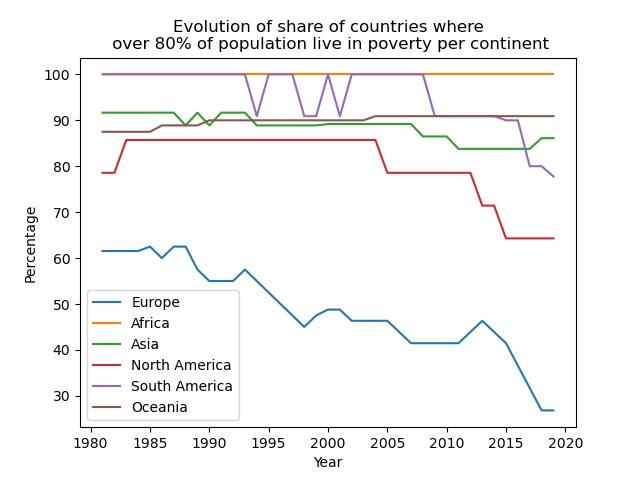
\includegraphics[width=0.8\linewidth]{reports/assignment-1/imgs/plot.png}
        \caption{Plot on poverty per continent}
        \label{fig:plot}
    \end{figure}
\end{enumerate}

\newpage
\bibliography{refs}

\end{document}
